\documentclass[10pt,oneside]{article}

\usepackage[T1]{fontenc}
\usepackage{fontawesome}

\usepackage[paper=a4paper,margin=2cm,bottom=2.5cm]{geometry}
\usepackage[sfdefault,light,condensed]{roboto}
\usepackage[export]{adjustbox}
\usepackage[usenames,dvipsnames,table]{xcolor}

\usepackage{amsmath,amssymb,array,fancyhdr,graphicx,enumitem,lastpage,multicol,tabularx,textcomp,titlesec}
\usepackage{mathtools}

\setlength\extrarowheight{1pt}
\setlength\parindent{0cm}
\renewcommand\headrule{}
\setlength{\footskip}{1.25cm}

\pagestyle{fancy}

\definecolor{BoxHeaderBG}{RGB}{50, 50, 50}
\definecolor{BoxHeaderText}{RGB}{255, 255, 255}

\newcommand{\BoxHeader}[2]{
    \multicolumn{#1}{| >{\bfseries\footnotesize\cellcolor{BoxHeaderBG}\arraybackslash}l |}{
        \textcolor{BoxHeaderText}{#2}
    }
}

\definecolor{ATLHeaderBG}{RGB}{65, 190, 30}
\definecolor{ATLHeaderText}{RGB}{0, 0, 0}

\definecolor{ATLSkillBG}{RGB}{215, 230, 210}
\definecolor{ATLSkillText}{RGB}{0, 0, 0}

\definecolor{DefinitionBoxHeaderBG}{RGB}{30, 30, 110}
\definecolor{DefinitionBoxHeaderText}{RGB}{255, 255, 255}

\definecolor{FormativeHeaderBG}{RGB}{150, 30, 150}
\definecolor{FormativeHeaderText}{RGB}{255, 255, 255}

\definecolor{GlobalContextHeaderBG}{RGB}{255, 255, 150}
\definecolor{GlobalContextHeaderText}{RGB}{0, 0, 0}

\definecolor{KeyConceptHeaderBG}{RGB}{15, 225, 225}
\definecolor{KeyConceptHeaderText}{RGB}{0, 0, 0}

\definecolor{RelatedConceptHeaderBG}{RGB}{15, 170, 170}
\definecolor{RelatedConceptHeaderText}{RGB}{0, 0, 0}

\definecolor{QuestionHeaderBG}{RGB}{240, 240, 240}
\definecolor{QuestionHeaderText}{RGB}{0, 0, 0}

\definecolor{SolutionHeaderBG}{RGB}{225, 150, 110}
\definecolor{SolutionHeaderText}{RGB}{0, 0 , 0}

\definecolor{SummativeHeaderBG}{RGB}{195, 15, 15}
\definecolor{SummativeHeaderText}{RGB}{255, 255, 255}

\newcommand{\ATLHeader}[1]{
    \cellcolor{ATLHeaderBG}\textcolor{ATLHeaderText}{
        \bfseries\footnotesize
        ATL SKILL (#1) \hfill \faGears
    }
}

\newcommand{\ATLSkill}[1]{
    \cellcolor{ATLSkillBG}\textcolor{ATLSkillText}{
        \itshape #1
    }
}

\newcommand{\DefinitionBoxHeader}{
    \cellcolor{DefinitionBoxHeaderBG}\textcolor{DefinitionBoxHeaderText}{
        \bfseries\footnotesize
        DEFINITIONS \hfill \faPencil
    }
}

\newcommand{\FormativeHeader}{
    \cellcolor{FormativeHeaderBG}\textcolor{FormativeHeaderText}{
        \bfseries\footnotesize
        FORMATIVE ASSESSMENT \hfill \faComments
    }
}

\newcommand{\GlobalContextHeader}[1]{
    \cellcolor{GlobalContextHeaderBG}\textcolor{GlobalContextHeaderText}{
        \bfseries\footnotesize
        GLOBAL CONTEXT (#1) \hfill \faGlobe
    }
}

\newcommand{\KeyConceptHeader}[1]{
    \cellcolor{KeyConceptHeaderBG}\textcolor{KeyConceptHeaderText}{
        \bfseries\footnotesize
        KEY CONCEPT (#1) \hfill \faKey
    }
}

\newcommand{\RelatedConceptHeader}[1]{
    \cellcolor{RelatedConceptHeaderBG}\textcolor{RelatedConceptHeaderText}{
        \bfseries\footnotesize
        RELATED CONCEPT (#1) \hfill \faLink
    }
}

\newcommand{\SolutionHeader}[1]{
    \cellcolor{SolutionHeaderBG}\textcolor{SolutionHeaderText}{
        \bfseries\footnotesize 
        #1 \hfill \faPaste
    }
}

\newcommand{\SummativeHeader}{
    \cellcolor{SummativeHeaderBG}\textcolor{SummativeHeaderText}{
        \bfseries\footnotesize
        SUMMATIVE ASSESSMENT \hfill \faCheck
    }
}

\newcounter{QuestionCounter}

\newcommand{\QuestionBox}[1]{
    \stepcounter{QuestionCounter}
    \cellcolor{QuestionHeaderBG}\textcolor{QuestionHeaderText}{
        {\bfseries\scriptsize Q\theQuestionCounter} #1
    }
}

\newcommand{\boxwidth}{\linewidth}

\lhead{\scriptsize\texttt{U\UnitNumber: \UnitTitle \\ L\LessonNumber: \LessonTitle}}
\rhead{\scriptsize\ttfamily [DESIGN/\CourseName/U\UnitNumber/L\LessonNumber]\\\ }

\lfoot{
\includegraphics[height=2cm,valign=c]{Files/logo}}
\cfoot{\footnotesize DESIGN/\CourseName/U\UnitNumber/L\LessonNumber\ | \LessonTitle \\ Woodstock School | Mussoorie, Uttarakhand, India}
\rfoot{
\includegraphics[height=2cm,valign=c]{Files/ib-world-school-logo-1-colour}}

\titleformat{\section}{\normalfont\Large\bfseries}{}{0em}{}[{\titlerule[0.5pt]}]
\titleformat{\subsection}{\normalfont\large\bfseries}{}{0em}{}


\usepackage{circuitikz,subcaption}
\usetikzlibrary{arrows,calc}

\def\CourseName{MYP3}

\def\LessonNumber{02}
\def\LessonTitle{Measuring Electricity}

\def\UnitNumber{01}
\def\UnitTitle{Circuits \& Electronics}

\begin{document}
    % Core Components (Remove when no longer required!)
    \thispagestyle{empty}
    \begin{tabularx}{\boxwidth}{| X | }
        \hline
        \ATLHeader{} \\\hline
        \ATLSkill{} \\\hline
        \QuestionBox{} \\\hline
    \end{tabularx}

    \begin{tabularx}{\boxwidth}{| X |}
        \hline
        \DefinitionBoxHeader \\\hline
    \end{tabularx}

    \begin{tabularx}{\boxwidth}{| X |}
        \hline
        \GlobalContextHeader{}\\\hline
    \end{tabularx}

    \begin{tabularx}{\boxwidth}{| X |}
        \hline
        \KeyConceptHeader{} \\\hline
    \end{tabularx}

    \begin{tabularx}{\boxwidth}{| X |}
        \hline
        \RelatedConceptHeader{} \\\hline
    \end{tabularx}

    \begin{tabularx}{\boxwidth}{| X |}
        \hline
        \SolutionHeader{SOLUTION} \\\hline
    \end{tabularx}

    \begin{tabularx}{\boxwidth}{| X | }
        \hline
        \FormativeHeader \\\hline
        \QuestionBox{} \\\hline
    \end{tabularx}

    \begin{tabularx}{\boxwidth}{| X |}
        \hline
        \SummativeHeader \\\hline
        \QuestionBox{}\\\hline
    \end{tabularx}

    \newpage

    \begin{center}
        \huge\bfseries
        \LessonTitle
    \end{center}

    \section{Before You Begin}

    \begin{tabularx}{\boxwidth}{| X |}
        \hline
        \KeyConceptHeader{Development} \\\hline
    \end{tabularx}

    \begin{tabularx}{\boxwidth}{| X |}
        \hline
        \RelatedConceptHeader{Invention} \\\hline
        \QuestionBox{We are examining the invention of electrical circuits as a \emph{turning point} in history. What other inventions do you think resulted in an historical turning point?} \\\hline
        \ \\[3cm]\hline
    \end{tabularx}
    \pagebreak

    \section{Technical Background}
    This lesson will be primarily concerned with the way we measure electricity within our circuits, and how we can select appropriate components based on the amount of electricity supplied and/or required.

    \subsection{Voltage}
    Voltage, measured in \emph{volts} (\textbf{V}), is a \emph{potential} difference between a positively and negatively charged part of a circuit. A common example illustrating the concept of voltage that of a water tank or tower.

    \begin{figure}[h]
        \centering
        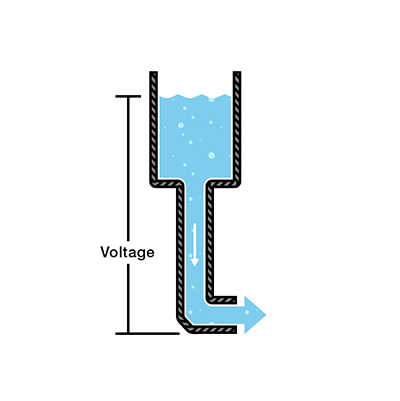
\includegraphics[height=6cm]{Extras/voltage}
        \caption*{\small Image courtesy sparkfun.com.}
    \end{figure}
    In this illustration, voltage can be seen as equivalent to the \emph{water pressure} coming out of the hose at the bottom of the system. Factors such as the height and size of the tank can have an impact on how much pressure is available. This is the \emph{potential energy} concept. While batteries and other sources of electricity provide power in different ways, the analogy is still useful for understanding what voltage contributes to an electrical circuit.

    \subsubsection*{Voltage Drop / Forward Voltage} 
    \emph{Voltage Drop} or \emph{Forward Voltage} is the amount of voltage required to power a load or other component in an electrical circuit.

    \medskip
    \begin{tabularx}{\boxwidth}{| X |}
        \hline
        \SolutionHeader{Kirchhoff's Voltage Law} \\\hline
        \emph{Kirchhoff's Voltage Law} (or \emph{Kirchhoff's Second Law}) essentially states that sum of all voltage drops in a closed electrical circuit, such as the simple circuits we built in the previous lesson, will be equal to the voltage of the source.\\\hline
    \end{tabularx}

    \subsection{Current}
    Current, measured in \emph{amperes} (\textbf{A}), is the \emph{flow} of electricity within a circuit. You can think of current as the \emph{speed} at which electricity flows.    

    \medskip
    \begin{tabularx}{\boxwidth}{| X | }
        \hline
        \ATLHeader{Communication Skills} \\\hline
        \ATLSkill{...make inferences and draw conclusions...} \\\hline
        \QuestionBox{Considering the water tank example given above for voltage, what changes to the system would have an impact on the flow of water out of it?} \\\hline
        \ \\[4cm]\hline
    \end{tabularx}

    \subsubsection*{Forward Current}
    Similar to forward voltage, forward current is the amount of current required by a load or component to work properly. As we will see later, the \emph{maximum} forward current is often supplied by device manufacturers, which indicates how much current the device or component can handle before becoming damanged. This value will have a significant impact on how we design our circuits.

    \medskip
    {\small\textbf{Note:} One ampere (\textbf{1A}) represents a significant amount of current for our simple components. Because of this, we will often discuss maximum forward current in terms of milliamperes (\textbf{mA}), or ``milliamps''. One milliamp represents $\frac{1}{1000}$ of an ampere.
    
    \medskip
    \textbf{Example:} A typical maximum forward current we will see is \textbf{20mA}. This represents $\frac{20}{1000}$, or \textbf{0.02A}.
    }

    \subsection{Resistance}
    Resistance, measured in Ohms ($\mathbf{\Omega}$), is a property of different materials to resist the flow of electricity within a circuit.

    \subsubsection*{Conductor v. Insulator}
    Materials can be divided into two broad categories: conductors and insulators. A \emph{conductor} offers little resistance to the flow of electricity, while an \emph{insulator} provides significant resistance. For example, copper wire is a conductor while most plastics are insulators. 
    
    \begin{figure}[h]
        \centering
        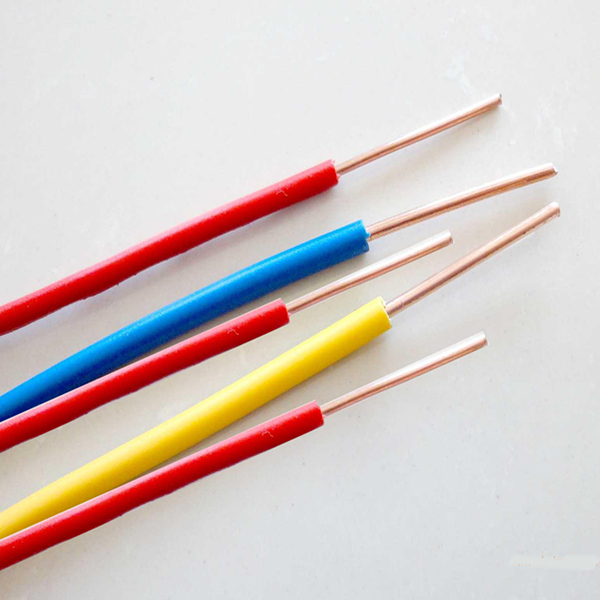
\includegraphics[height=4cm]{Extras/copper_wire}
        \caption*{\small Image courtesy of sparkfun.com.}
    \end{figure}

    The above image shows a copper wire that has been stripped of some of its plastic sheath insulation.

    \medskip
    \begin{tabularx}{\boxwidth}{| X | }
        \hline
        \ATLHeader{Communication Skills} \\\hline
        \ATLSkill{...make inferences and draw conclusions...} \\\hline
        \QuestionBox{Why do conductive wires often get wrapped in an insulating material, like in the image above?} \\\hline
        \ \\[3cm]\hline
        \QuestionBox{Many of the components we are going to be using are made using a \emph{semiconductor} material. How do you think semiconductors compare to conductors and insulators?} \\\hline
        \ \\[3cm]\hline
    \end{tabularx}

    \subsection{Ohm's Law}
    \begin{tabularx}{\boxwidth}{| X |}
        \hline
        \SolutionHeader{Ohm's Law} \\\hline
        \emph{Ohm's Law} provides us with a very simple formula linking voltage (\textbf{V}), current (\textbf{I}), and resistance (\textbf{R}):\\
        \[ V = IR \hspace*{2cm} \text{OR} \hspace*{2cm} I = \frac{V}{R} \hspace*{2cm} \text{OR} \hspace*{2cm} R = \frac{V}{I} \]\\\hline
    \end{tabularx}

    % Ohm's Law

    \subsection{The Resistor}

    \begin{tabularx}{\boxwidth}{| >{\bfseries}p{0.15\boxwidth} | X | >{\centering\arraybackslash}p{0.15\boxwidth} | >{\centering\arraybackslash}p{0.15\boxwidth}| }
        \hline
        \BoxHeader{1}{Name} & \BoxHeader{1}{Description} & \BoxHeader{1}{Symbol} & \BoxHeader{1}{Example} \\\hline
        Resistor & 
        A \emph{resistor} is an electronic component specifically designed to reduce the current flow in a circuit.

        \medskip
        The \emph{resistance} offered by each resistor is measured in Ohms ($\Omega$).
        & 
        \raisebox{-0.5cm}{
            {\tikz \draw (0, 0) to [R] (2, 0);} 
        }

        \bigskip
        {\tikz \draw (0, 0) to [european resistor] (2, 0);}
        & 
        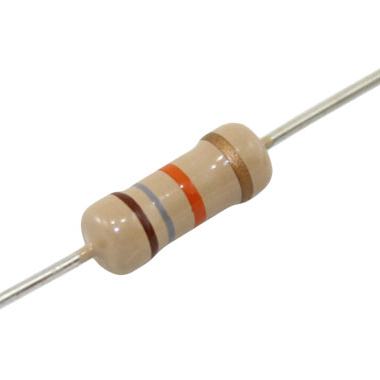
\includegraphics[width=0.9\boxwidth,valign=t]{Extras/resistor}
        \\\hline
    \end{tabularx}

    \medskip
    The type of resistor we will be using are labeled using coloured bands to denote their resistance. You have a copy of the following image in your electronics kits:
    
    \begin{figure}[h]
        \centering
        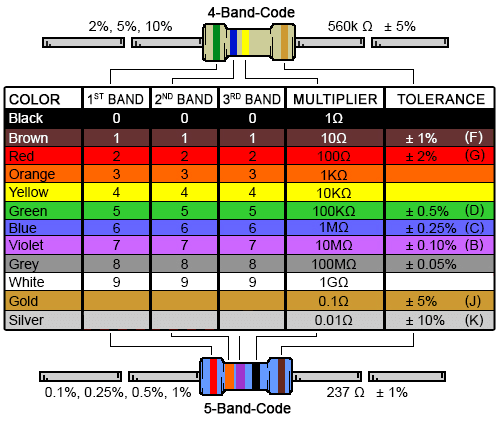
\includegraphics[height=8cm]{Extras/resistor_chart}
        \caption*{\small Image courtesy digikey.com.}
    \end{figure}

    \begin{tabularx}{\boxwidth}{| X |}
        \hline
        \ATLHeader{Communication Skills} \\\hline
        \ATLSkill{...use and interpret a range of discipline-specific terms and symbols...} \\\hline
        \QuestionBox{Throughout this course, we will be using a variety of different resistors. The following resistance value resistors are quite common: $220 \Omega$, $1 \text{k}\Omega$, $10 \text{k}\Omega$. These are available in your electronics kit. Determine whether your resistors are $4-$ or $5-$band and identify the correct colour bands for each required value. You can safely ignore the ``tolerance'' band for now.} \\\hline

        \textbf{220 $\mathbf{\Omega}$ \hfill 1 k$\mathbf{\Omega}$ \hfill 10 k$\mathbf{\Omega}$ \hspace{4cm} \,} \\[4cm]\hline
    \end{tabularx}

    \pagebreak

    \section{Developing Technical Skills}
    % ! Circuit #1:
    % ! -- Simple circuit #2 with a 9-volt battery
    % ! -- What happens?
    % ! Look @ Data Sheet
    % ! -- Finding data sheets.
    % ! -- Looking for relevant information.
    % Circuit #2:
    % -- Simple circuit with appropriate resistor & 9-volt battery.
    % -- Calculating required resistance.

    \subsection{Circuit \#4: Higher Voltages}
    This circuit usees a 9-volt battery to examine how voltage impacts the performance of circuit components. Note that you might need to hold the 9-volt battery in place. If this is proving difficult, team up with a partner who can help you operate the circuit with the battery properly positioned.

    \subsubsection*{You Will Need:}
    \begin{itemize}[noitemsep]\small
        \item (1) 9V Battery
        \item (1) LED
        \item (1) Pushbutton
        \item (1) Roll of Copper Tape
        \item (1) Roll of Cellophane Tape
    \end{itemize}

    \subsubsection*{Directions}
    Create the following paper circuit. Note the position of the different sized terminals on the 9V battery.

    \begin{center}
        \newdimen\R
        \R=0.38cm
        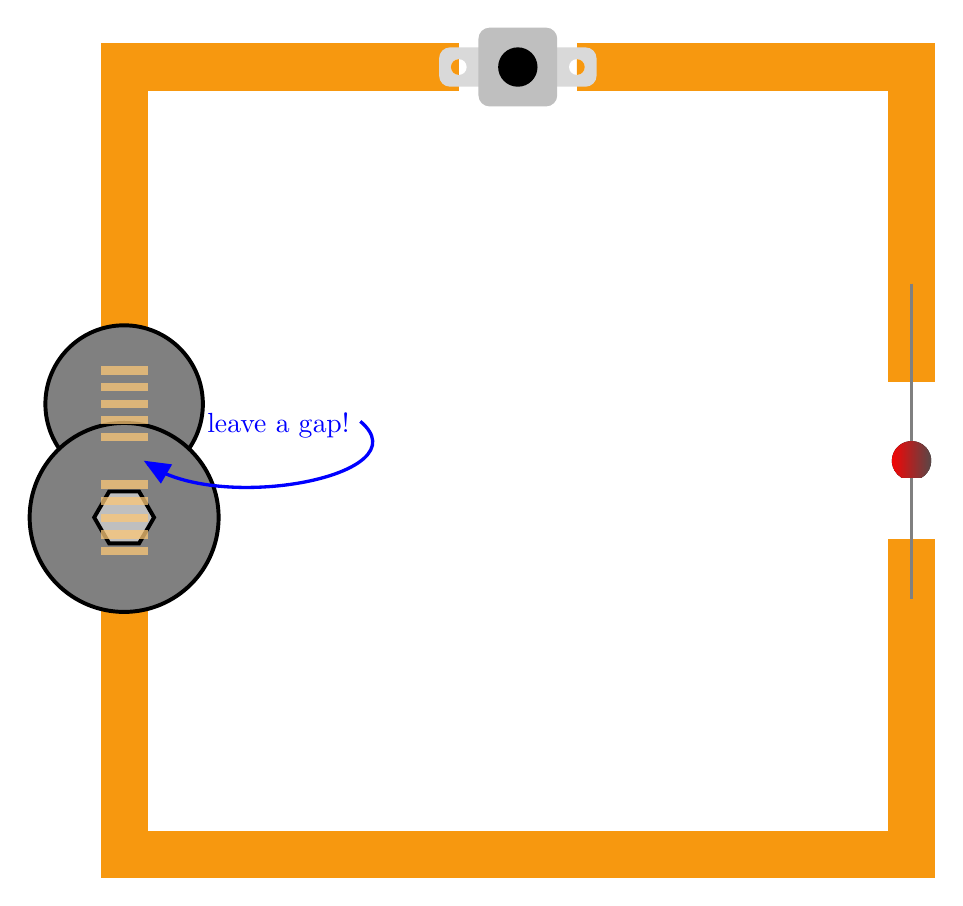
\begin{tikzpicture}

            \draw[line width=6mm,YellowOrange] (0, 0) -- (0, 5) -- (4.25, 5);
            \draw[line width=6mm,YellowOrange] (5.75, 5) -- (10, 5) -- (10, 1);
            \draw[line width=6mm,YellowOrange] (10, -1) -- (10, -5) -- (0, - 5) -- (0, 0);

            % 9-Volt Battery:
            \filldraw[fill=black!25,rounded corners] (-0.845, -1.3) rectangle (0.845, 1.3);
            

            \draw[fill=black!50,line width=0.5mm] (0, 0.72) circle (\R);
            \draw[fill=black!50,line width=0.5mm] (0, -0.72) circle (1.2\R);
            \begin{scope}[yshift=-0.72cm]
                \draw[fill=black!25,line width=0.5mm] (0:0.38) \foreach \x in {60,120,...,359} {
                    -- (\x:0.38)
                }-- cycle (90:0.38);
            \end{scope}

            \draw[line width=6mm,YellowOrange!50,dashed,draw opacity=0.75] (0, 0.25) -- (0, 1.3);     
            \draw[line width=6mm,YellowOrange!50,dashed,draw opacity=0.75] (0, -0.25) -- (0, -1.3);

            \draw[->,>=triangle 45,very thick, blue] (3, 0.5) node[anchor=south east,yshift=-10] {leave a gap!} to [out=-40,in=-40] (0.25, 0);

            % Pushbutton
            \fill[rounded corners,black!15] (4, 4.75) rectangle (6, 5.25);
            \fill[rounded corners,black!25] (4.5, 4.5) rectangle (5.5, 5.5);
            \fill[black] (5, 5) circle (0.25);
            \fill[white] (4.25, 5) circle (0.1);
            \fill[white] (5.75, 5) circle (0.1);
            \fill[YellowOrange] ([shift=(90:1mm)]4.25, 5) arc (90:270:1mm);
            \fill[YellowOrange] ([shift=(90:1mm)]5.75, 5) arc (90:-90:1mm);
        
            % LED
            \draw[very thick,black!50] (10, 2.25) -- (10, -1.75);    
            \fill[left color=red, right color=black!70] ([shift=(-60:2.5mm)]10,0) arc (-60:240:2.5mm);
        \end{tikzpicture}
    \end{center}

    \medskip
    \begin{tabularx}{\boxwidth}{| X | }
        \hline
        \ATLHeader{Communication Skills} \\\hline
        \ATLSkill{...make inferences and draw conclusions...} \\\hline
        \QuestionBox{What happens when you power the above circuit? Did you expect that to happen? Attempt an explanation based on the technical details discussed earlier, particularly the relationship between voltage and current.} \\\hline
        \ \\[3.5cm]\hline
    \end{tabularx}

    \pagebreak

    \subsection{Examining Datasheets}
    A \emph{datasheet} is a technical document listing important details about each specific component we will use in our circuits. While these had traditionally been packaged with purchased items, most of the time they are now just a quick Google search away.

    \medskip
    The following two images show first an overview of a datasheet for one of the red LEDs we have been using, then the specific area of the datasheet we will be interested in for this lesson.

    \medskip
    \begin{figure}[h]
        \hspace*{0.5cm}
        \begin{subfigure}{4cm}
            \centering
            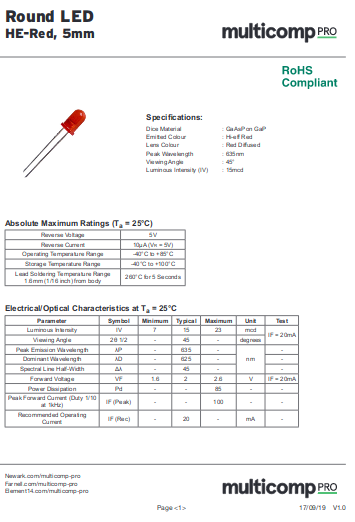
\includegraphics[width=3cm]{Extras/datasheet_whole}
            \caption*{\footnotesize\raggedright An overview of an entire datasheet, courtesy element14.com.}
        \end{subfigure}
        \hspace*{2cm}
        \begin{subfigure}{10cm}
            \centering
            \begin{tikzpicture}
             \node[anchor=south west] at (0, 0) {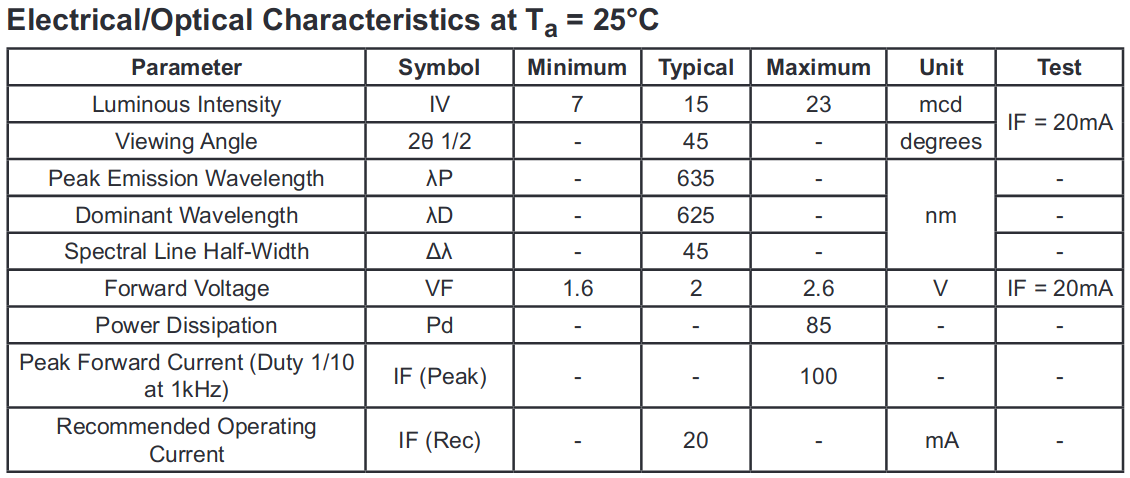
\includegraphics[width=9.75cm]{Extras/datasheet_part}};
            \fill[rounded corners, thick, yellow, fill opacity=0.2] (0.05, 0.1) rectangle (9.95, 0.8);
            \fill[rounded corners, thick, yellow, fill opacity=0.2]  (0.05, 1.55) rectangle (9.95, 2);
            \end{tikzpicture} 
      \caption*{\footnotesize A zoom in on the ``Electrical Characteristics'' portion of the datasheet, with required details highlighted.}
        \end{subfigure}
    \end{figure}

    \begin{tabularx}{\boxwidth}{| X |}
        \hline
        \ATLHeader{Communication Skills} \\\hline
        \ATLSkill{...use and interpret a range of discipline-specific terms and symbols...} \\\hline
        \QuestionBox{Using the information in the data sheet above, describe how \emph{Kirchhoff's Voltage Law} explains why your two LED circuit from Lesson \#1 did not function as intended.}\\\hline
        \ \\[4cm]\hline
        \QuestionBox{Later this unit, we will be using a ``BC547B Transistor''. Find a datasheet for this component online and determine the current and voltage associated with ``Small Signal Current Gain'' (h$_\text{fe}$).} \\\hline
        \ \\[4cm]\hline
    \end{tabularx}

    \pagebreak
    \subsection{Circuit \#5: Using Resistors}
    The following circuit solves the problem experienced in Circuit \#4 by introducing a \emph{resistor}. This will lower the current passing through the LED to below its maximum forward currrent rating (20 mA).

    \subsubsection*{You Will Need:}
        \begin{itemize}[noitemsep]
            \item (1) 9V Battery
            \item (1) LED
            \item (1) Pushbutton
            \item (1) Resistor (Yellow-Violet-Brown)
            \item (1) Roll of Copper Tape
            \item (1) Roll of Cellophane Tape
        \end{itemize}

    \subsubsection*{Directions:}
    Create the following paper circuit. Note that unlike the LED, a resistor is \emph{bidirection}; it does not need to be placed in any particular way.

    \begin{center}
        \newdimen\R
        \R=0.38cm
        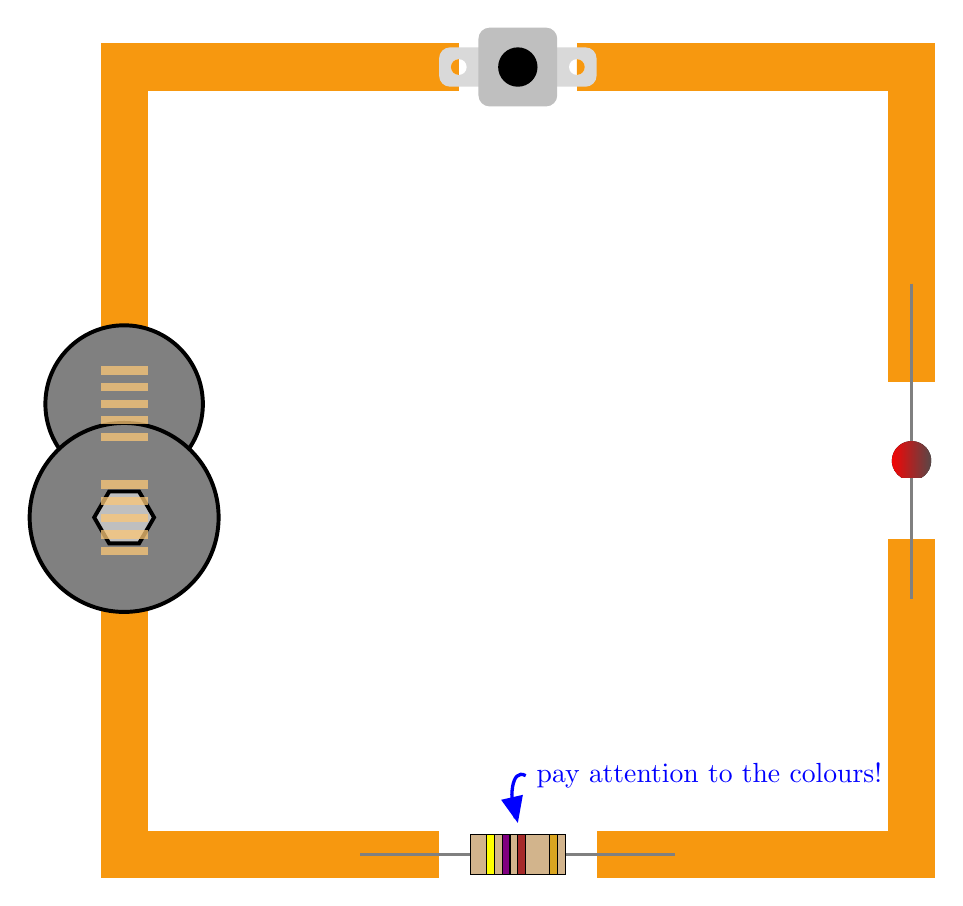
\begin{tikzpicture}

            \draw[line width=6mm,YellowOrange] (0, 0) -- (0, 5) -- (4.25, 5);
            \draw[line width=6mm,YellowOrange] (5.75, 5) -- (10, 5) -- (10, 1);
            \draw[line width=6mm,YellowOrange] (10, -1) -- (10, -5) -- (6, -5);
            \draw[line width=6mm,YellowOrange] (4, -5) -- (0, -5) -- (0, 0);

            % 9-Volt Battery:
            \filldraw[fill=black!25,rounded corners] (-0.845, -1.3) rectangle (0.845, 1.3);
            

            \draw[fill=black!50,line width=0.5mm] (0, 0.72) circle (\R);
            \draw[fill=black!50,line width=0.5mm] (0, -0.72) circle (1.2\R);
            \begin{scope}[yshift=-0.72cm]
                \draw[fill=black!25,line width=0.5mm] (0:0.38) \foreach \x in {60,120,...,359} {
                    -- (\x:0.38)
                }-- cycle (90:0.38);
            \end{scope}

            \draw[line width=6mm,YellowOrange!50,dashed,draw opacity=0.75] (0, 0.25) -- (0, 1.3);     
            \draw[line width=6mm,YellowOrange!50,dashed,draw opacity=0.75] (0, -0.25) -- (0, -1.3);

            % Pushbutton
            \fill[rounded corners,black!15] (4, 4.75) rectangle (6, 5.25);
            \fill[rounded corners,black!25] (4.5, 4.5) rectangle (5.5, 5.5);
            \fill[black] (5, 5) circle (0.25);
            \fill[white] (4.25, 5) circle (0.1);
            \fill[white] (5.75, 5) circle (0.1);
            \fill[YellowOrange] ([shift=(90:1mm)]4.25, 5) arc (90:270:1mm);
            \fill[YellowOrange] ([shift=(90:1mm)]5.75, 5) arc (90:-90:1mm);
        
            % LED
            \draw[very thick,black!50] (10, 2.25) -- (10, -1.75);    
            \fill[left color=red, right color=black!70] ([shift=(-60:2.5mm)]10,0) arc (-60:240:2.5mm);

            % Resistor (requires calc library)
            \coordinate (R1) at (3, -5);
            \draw[very thick, black!50] (R1) -- ($(R1) + (4, 0)$);
            \draw[fill=Tan ] ($(R1) + (1.4, 0.25)$) rectangle ($(R1) + (2.6, -0.25)$);
            \draw[fill=Yellow] ($(R1) + (1.6, 0.25)$) rectangle ($(R1) + (1.7, -0.25)$);
            \draw[fill=Purple] ($(R1) + (1.8, 0.25)$) rectangle ($(R1) + (1.9, -0.25)$);
            \draw[fill=Brown] ($(R1) + (2.0, 0.25)$) rectangle ($(R1) + (2.1, -0.25)$);
            \draw[fill=Goldenrod] ($(R1) + (2.5, 0.25)$) rectangle ($(R1) + (2.4, -0.25)$);

            \draw[->,>=triangle 45,blue,very thick] (5.1, -4) node[anchor=west] {pay attention to the colours!} to [in=120,out=150] (5, -4.6);
        \end{tikzpicture}
    \end{center}

    \bigskip\bigskip
    \begin{tabularx}{\boxwidth}{| X | }
        \hline
        \ATLHeader{Communication Skills} \\\hline
        \ATLSkill{...use and interpret a range of discipline-specific termas and symbols...} \\\hline
        \QuestionBox{What is the value of the resistor used in this circuit? Use your resistor colour band chart as reference.} \\\hline
        \ \\[3cm]\hline
    \end{tabularx}

    \pagebreak

    \subsection{Finding the Perfect Resistor}
    The following process shows how we can determine what the appropriate resistor is for our simple circuits.

    \begin{minipage}[t]{0.45\boxwidth}\vspace{0pt}
        {\bfseries Step 1:}

        \bigskip
        \begin{minipage}{0.5\boxwidth}
            \begin{circuitikz}[scale=0.9]
                \draw (0, 1) node[left] {+} to [battery] (0, 0);
                \draw (0, 1) |- (1, 2) to [push button] (2, 2) -| (3, 1) to [full led] (3, 0) |- (2, -1) to [european resistor] (1, -1) -| (0, 0);
                \node at (2.4, 0.5) {\textbf{\textcolor{Blue}{\small 2V}}};
                \node at (1.5, -0.5) {\textbf{\textcolor{Blue}{\small ???}}};
            \end{circuitikz}
        \end{minipage}
        \begin{minipage}{0.05\boxwidth}
            \ 
        \end{minipage}
        \begin{minipage}{0.4\boxwidth}
            \large
            V$_{\text{R}} =  \text{V}_{\text{S}} -  \text{V}_{\text{L}}$ \\
            V$_{\text{R}} = 9 - 2$\\
            V$_{\text{R}} = 7$\\
        \end{minipage}\\

        \medskip
        Determine the voltage drop across the resistor by using \emph{Kircchoff's Voltage Law.} Remember: the total of the forward voltages across all components should be equal to the source voltage. The LED's voltage comes from its datasheet.
    \end{minipage}
    \begin{minipage}[t]{0.05\boxwidth}\vspace{0pt}
        \ 

    \end{minipage}
    \begin{minipage}[t]{0.45\boxwidth}\vspace{0pt}
        {\bfseries Step 2:}

        \bigskip
        \begin{circuitikz}[scale=0.9]
            \draw (0, 1) node[left] {+} to [battery] (0, 0);
            \draw (0, 1) |- (1, 2) to [push button] (2, 2) -| (3, 1) to [full led] (3, 0) |- (2, -1) to [european resistor] (1, -1) -| (0, 0);
            \node at (2.5, 0.5) {\textbf{\textcolor{Blue}{\small 2V}}};
            \node at (1.5, -0.5) {\textbf{\textcolor{Blue}{\small 7V}}};
            \draw[->,>=triangle 45,thick,red] (1.5, 0.5) +(180:0.75) arc (180:-170:0.75);
            \node at (1.5, 0.5) {\textbf{\textcolor{Red}{\small ???}}};
        \end{circuitikz}

        \medskip
        Determine the \emph{desired} current. This is the maximum forward current from the LEDs datasheet (20 mA or 0.02A).

    \end{minipage}

    \bigskip
    \begin{minipage}[t]{0.45\boxwidth}\vspace{0pt}
        {\bfseries Step 3:}

        \bigskip
        \begin{minipage}{0.5\boxwidth}
            \begin{circuitikz}[scale=0.9]
                \draw (0, 1) node[left] {+} to [battery] (0, 0);
                \draw (0, 1) |- (1, 2) to [push button] (2, 2) -| (3, 1) to [full led] (3, 0) |- (2, -1) to [european resistor] (1, -1) -| (0, 0);
                \node at (2.5, 0.5) {\textbf{\textcolor{Blue}{\small 2V}}};
                \node at (1.5, -0.5) {\textbf{\textcolor{Blue}{\small 7V}}};
                \draw[->,>=triangle 45,thick,red] (1.5, 0.5) +(180:0.75) arc (180:-170:0.75);
                \node at (1.5, 0.5) {\textbf{\textcolor{Red}{\small 0.02A}}};
            \end{circuitikz} 
        \end{minipage}
        \begin{minipage}{0.05\boxwidth}
            \ 
            
        \end{minipage}
        \begin{minipage}{0.4\boxwidth}
            \large
            R $= \dfrac{\text{V}}{\text{I}}$ \\

            \smallskip
            R $= \dfrac{7}{0.02}$ \\

            \smallskip
            R $= 345$
        \end{minipage}\\

        \bigskip\medskip
        Apply \emph{Ohm's Law} to calculate the resistance required across the resistor in the circuit.
    \end{minipage}
    \begin{minipage}[t]{0.05\boxwidth}\vspace{0pt}
        \ 

    \end{minipage}
    \begin{minipage}[t]{0.45\boxwidth}\vspace{0pt}
        {\bfseries Step 4:}

        \bigskip
        \begin{circuitikz}[scale=0.9]
            \draw (0, 1) node[left] {+} to [battery] (0, 0);
            \draw (0, 1) |- (1, 2) to [push button] (2, 2) -| (3, 1) to [full led] (3, 0) |- (2, -1) to [european resistor] (1, -1) -| (0, 0);
            %\node at (2.25, 0.5) {\textbf{\textcolor{Blue}{2V}}};
            %\node at (1.5, -0.5) {\textbf{\textcolor{Blue}{???}}};
            \node at (1.5, -1.5) {\textbf{\textcolor{Green}{345 $\Omega$}}};
        \end{circuitikz}

        \medskip
        Typical circuit diagrams will include the resistor value as a label on each resistor.
    \end{minipage}

    \bigskip\bigskip
    \begin{tabularx}{\boxwidth}{| X | }
        \hline
        \ATLHeader{Communication Skills} \\\hline
        \ATLSkill{...make inferences and draw conclusions...} \\\hline
        \QuestionBox{Why do you think we don't assign a forward voltage to the push button in our circuits?} \\\hline
        \ \\[3cm]\hline
        \QuestionBox{Despite the appropriate resistor is calculated as having a value of $345 \Omega$, this is \emph{not} the resistor we used in Circuit \#5. Why do you think we chose a larger valued resistor for this circuit?} \\\hline
        \ \\[3cm]\hline
    \end{tabularx}
    
    \pagebreak
    \section{Reflections}
\end{document}